% Verbatim from minor_report/chapters/chapter_4_results.tex lines 82-912 (retired report),
% headings demoted by 1 level(s). Do not edit here; edit the source of the numbers.

\subsubsection{Question, hypotheses, and conditions}

Until this experiment, every trajectory figure in this chapter reported visual
error against ground truth with nothing to compare it to, so a reader could see
how large the error was but not whether it was good. This section establishes the
dead-reckoning floor. The question is whether a non-visual estimator---wheel
odometry, IMU dead reckoning, or an EKF fusing them---provides usable
localization on the same recorded data, and whether the uncertainty each one
reports describes the error it actually makes.

Four hypotheses were registered before the metrics were computed:
\begin{itemize}
  \item[H1] Wheel-odometry drift is dominated by the measured yaw-rate scale
    error, so the two bags, whose scales err $+1.1\%$ and $-4.7\%$, should bow in
    opposite rotational directions.
  \item[H2] IMU-only dead reckoning diverges by orders of magnitude more than
    wheel odometry over the same interval.
  \item[H3] The EKF improves on both single-sensor estimators.
  \item[H4] All three report overconfident covariances, because a dead-reckoning
    noise model omits systematic scale error.
\end{itemize}

The independent variable is the estimator; everything else is held fixed within a
dataset. \Cref{tab:proprio-controls} records the controlled conditions. All five
estimators consume the same recordings and all visual runs replayed them under
identical settings.

The five datasets are not repeats of one condition. Only \repo{allsensor_000} and
\repo{allsensor_001} share a world. The remaining three vary two factors: object
placement, where \texttt{objonwallonly} restricts obstacles to the wall region and
clears the central floor, and floor texture, where \texttt{bayline} adds painted
bay lines to a surface that is otherwise featureless. No quantity is pooled across
worlds; each dataset is read as its own condition.

\begin{table}[htbp]
\centering
\caption[Conditions for the estimator comparison.]{Conditions for the estimator comparison. All five estimators consume the
same five recordings and are scored against the same ground truth over the same
interval. One factor listed here is \emph{not} controlled and is marked as such:
the IMU noise model differs systematically between the proprioceptive and visual
families, and \cref{sec:proprio-tuning} measures what that is worth.}
\label{tab:proprio-controls}
\small
\begin{tabularx}{\textwidth}{>{\raggedright\arraybackslash}p{0.26\textwidth}>{\raggedright\arraybackslash}X}
\toprule
Factor & Level \\
\midrule
Worlds & four: \repo{..._static_01_nofloortexture} (000, 001),
  \repo{..._static_nofloortexture_objonwallonly} (002),
  \repo{..._static_bayline_objonwallonly} (003),
  \repo{..._static_01_bayline} (004) \\
Floor & plain (000--002) versus bayline, i.e.\ painted lines (003, 004) \\
Scene dynamics & static \\
Floor & featureless \\
Datasets & five, \SIrange{81.8}{102.4}{\second} of simulated time and
  \SIrange{113.1}{142.3}{\metre} driven each \\
Dynamic filter & disabled in every run (\repo{filter=false}) \\
Replay rate & $0.5\times$ for both visual estimators \\
Ground truth & \repo{/ground_truth/odometry}, \SI{50}{\hertz}, header stamps \\
Alignment & rigid $SE(3)$, scale fixed, for cross-system comparison \\
IMU noise model & \flag{not controlled in this experiment.} The EKF's is measured
  per bag by \repo{proprio_estimator.py calibrate}; both visual estimators read
  four constants from \repo{config/wil_sim/stereo_imu.yaml}. The factor is
  confounded with the estimator here and is separated in
  \cref{sec:proprio-tuning} \\
Experimental unit, $n$ & one bag; $n=5$ across \emph{four} worlds. Only
  \texttt{static\_01} plain is repeated, and only twice \\
Visual configurations & VINS-Fusion; ORB-SLAM3 with loop closing enabled and
  disabled, one run each \\
\bottomrule
\end{tabularx}
\end{table}

\subsubsection{Validity}

\Cref{tab:proprio-accuracy} rests on thirty-five runs: three proprioceptive
baselines and the transferred-noise EKF of \cref{sec:proprio-tuning} on each of
the five bags, VINS-Fusion once per bag, and ORB-SLAM3 twice per bag for the two
loop-closure configurations. All thirty-five passed their predefined checks.

The proprioceptive baselines completed on all five bags with the planar
assumption holding by a wide margin---maximum tilt \SIrange{0.0015}{0.0018}{\degree}
against a \SI{1}{\degree} threshold---with the bicycle yaw-rate model selected
automatically on every bag, \repo{imu_orientation_used=NO} recorded in every run,
and the EKF applying 4\,355, 4\,091, 4\,338, 5\,120 and 5\,026 wheel corrections,
matching the wheel-odometry message counts exactly. VINS-Fusion processed every
image it received on all five.

\flag{The initialization and reset figures below were extracted for
\repo{allsensor_000} and \repo{allsensor_001} only and have not been recovered for
the other three bags:} VINS-Fusion initialized once in \SI{0.33}{\second} with no
resets, and both ORB-SLAM3 runs shut down gracefully with no tracking-loss events
and inertial initialization at \SI{2.48}{\second} and \SI{2.51}{\second}. Neither
\repo{run_metadata.csv} schema records initialization time, reset count or
tracking-loss events, so these cannot be recovered from the run record and would
have to be re-read from the console logs.

\begin{queried}[Queried]
ORB-SLAM3 receives fewer stereo pairs than are available on every dataset, while
VINS-Fusion receives all of them (2639, 2478 of 2479, 2628, 3102 and 3046). The
ORB shortfall is \SIrange{3.8}{11.9}{\percent} and varies by run as well as by
dataset: \SI{90.2}{\percent} and \SI{94.2}{\percent} of the available pairs on
\repo{allsensor_000} for the two configurations, \SI{96.2}{\percent} and
\SI{95.1}{\percent} on \repo{allsensor_003}. Its own counters report zero decode
failures, and the stereo timestamps are aligned to \SI{0}{\second} median offset
with \SI{100}{\percent} of pairs inside the \SI{20}{\milli\second} synchronisation
slop, so synchronisation is not what loses them.

The counter itself cannot say where they go: \repo{stereo_pairs_received} is
incremented inside the \emph{synchronised} callback, and the node keeps no count of
images arriving. What the source does show is an asymmetry in input buffering.
ORB-SLAM3 subscribes with \repo{rclcpp::SensorDataQoS()}, which is best-effort with
a depth of five, so a frame arriving while the tracking callback is busy is
discarded by the middleware and never recorded anywhere; VINS-Fusion subscribes
with \repo{KeepLast(100).reliable()} and buffers the same burst. \moved{The shortfall
is therefore most consistent with ORB-SLAM3 dropping frames at its own subscriber
under load, not with loss in transport.} The loop-closure-free runs support that
reading on three datasets, receiving more pairs than the enabled runs on
\repo{allsensor_000}, \repo{_001} and \repo{_002} while doing less work per frame,
though \repo{allsensor_003} runs the other way and the mechanism is not proven.
Trajectory accuracy over a shared interval is not obviously affected---ORB-SLAM3
is the more accurate of the two on some datasets despite the shortfall---but no
throughput, latency or per-frame compute comparison between the two estimators is
admissible until the loss is explained: the two estimators differ not only in
load but in input-queue policy, so such a comparison would measure the QoS choice
as much as the algorithm.
\end{queried}

\begin{queried}[Ruled out]
A plausible reading of these results is that the visual estimators lose to the EKF
because their input rate collapsed. The data does not support it. Source imagery
is regular at \SI{30.3}{\hertz} in simulated time on all five bags, with a median
inter-frame interval of \SI{0.0330}{\second} and no gap exceeding
\SI{0.1}{\second}; VINS-Fusion received and processed every frame on every
dataset, with zero skipped before the back end, and still trails the
cross-validated EKF on four of five. Frame loss is real for ORB-SLAM3 and remains
unexplained, but it cannot account for the margin, because the estimator with no
frame loss at all shows the same one.
\end{queried}

\begin{queried}[Queried]
ORB-SLAM3 was run in two configurations on every dataset, recorded as
\repo{logging_20260916_01} with loop closing enabled and
\repo{logging_20260916_02} with it disabled, and both are reported below as
separate systems. Within the enabled configuration the loop closer behaves very
differently per dataset (\cref{tab:orb-loop}), so those five trajectories are not
repeats of one condition and must not be pooled.

A counter reading \texttt{loop\_closures,0} does \emph{not} mean the loop closer
was inactive. On \repo{allsensor_000} it performed 447 place-recognition checks,
found 90 loop candidates and rejected all 90 on inertial geometry; on
\repo{allsensor_004} it found 114 and accepted none. The disabled runs are
distinguishable only in \repo{loop_closing.csv}, where every event carries
\texttt{current\_keyframe\_id}~$=-1$ and a duration below
\SI{0.003}{\milli\second}, the signature of a thread spinning with nothing queued
to it.
\end{queried}

\begin{table}[htbp]
\centering
\caption[Loop-closing activity in the enabled ORB-SLAM3 configuration (\repo{logging_20260916_01}).]{Loop-closing activity in the enabled ORB-SLAM3 configuration
(\repo{logging_20260916_01}). Accepted closures are a small and dataset-dependent
fraction of candidates, and two datasets accept none at all despite the closer
running throughout. In the disabled configuration
(\repo{logging_20260916_02}) no keyframe ever reaches the loop closer on any
dataset.}
\label{tab:orb-loop}
\small
\begin{tabular}{lrrrr}
\toprule
Dataset & Place-recognition events & Candidates & Accepted & Global BA \\
\midrule
\repo{allsensor_000} & 537 & 90 & 0 & 0 \\
\repo{allsensor_001} & 379 & 2 & 2 & 2 \\
\repo{allsensor_002} & 274 & 11 & 1 & 1 \\
\repo{allsensor_003} & 591 & 64 & 1 & 0 \\
\repo{allsensor_004} & 713 & 114 & 0 & 0 \\
\bottomrule
\end{tabular}
\end{table}

\begin{queried}[Provenance gap]
\repo{run_metadata.csv} records 22 parameters and loop-closure state is not among
them, so the whole distinction rests on the directory name---and that name does
not mean the same thing everywhere in this chapter. In the relogged campaign of
\cref{sec:results-validity}, \repo{logging_20260916_01} through \repo{_03} are
three \emph{repeats} of one configuration, all with an active loop closer. In the
\repo{allsensor} campaign reported here, \repo{_01} and \repo{_02} are two
\emph{configurations}, loop closing enabled and disabled, with one run each. The
same suffix therefore encodes a repeat index in one section and an experimental
factor in the next. The metadata for the two bag-000 runs is identical apart from the experiment
identifier, output path and start time, and both name the same installed
configuration file, so nothing in the recorded provenance distinguishes an
enabled run from a disabled one. The distinction used in this chapter was
recovered from \repo{loop_closing.csv} after the fact. The logger should record
the loop-closing and global-BA switches explicitly before any further ORB-SLAM3
campaign.
\end{queried}

\subsubsection{Accuracy results}

\Cref{tab:proprio-accuracy} reports all five estimators. Aligned ATE is the only
column comparable across systems, because the visual estimators build their own
world frames while the baselines start from the ground-truth pose.

\begin{table}[htbp]
\centering
\caption[Estimator comparison on the five \repo{allsensor} bags, which span four worlds and both floor conditions; they are not repeats of one another except for \repo{allsensor_000} and \repo{allsensor_001}.]{Estimator comparison on the five \repo{allsensor} bags, which span four
worlds and both floor conditions; they are not repeats of one another except for
\repo{allsensor_000} and \repo{allsensor_001}. Bold marks the best aligned ATE of
each dataset \emph{as each system was actually configured}---the EKF on four of
five, VINS-Fusion on \repo{allsensor_004}. That ranking is not tuning-controlled:
the EKF's noise model is measured from each bag, while both visual systems read
the hand-set \repo{config/wil_sim/stereo_imu.yaml}. The \emph{EKF @ VSLAM noise}
rows are the same filter on the same bags with only its four IMU noise terms
replaced by that file's values; it then loses to VINS-Fusion on all five bags
(\cref{sec:proprio-tuning}). ``Aligned ATE'' is
RMSE after a rigid $SE(3)$ fit with scale fixed, the convention used throughout
this chapter. ``Anchored'' columns are the direct difference from ground truth
with no alignment and are defined only for the estimators that start from the
ground-truth pose; the visual estimators' own world frames make that subtraction
meaningless, so those cells are set to --. Drift is the final position error as a
fraction of distance driven.}
\label{tab:proprio-accuracy}
\small
\setlength{\tabcolsep}{5pt}
\resizebox{\textwidth}{!}{%
\begin{tabular}{lllrrrrr}
\toprule
Dataset & World & Estimator & Aligned ATE & Anchored RMS & Anchored final &
  Drift & Final yaw \\
 & & & [\si{\metre}] & [\si{\metre}] & [\si{\metre}] & [\si{\percent}] &
  [\si{\degree}] \\
\midrule
\repo{allsensor_000} & \texttt{static\_01} & IMU dead reckoning & 21.697 & 39.353 &
  47.597 & 40.66 & $+2.19$ \\
 & plain & Wheel odometry & 2.801 & 4.732 & 4.767 & 4.07 & $-13.76$ \\
 & & VINS-Fusion & 0.616 & -- & -- & -- & -- \\
 & & ORB-SLAM3 & 0.579 & -- & -- & -- & -- \\
 & & ORB-SLAM3 (no LC) & 0.285 & -- & -- & -- & -- \\
 & & \textbf{EKF wheel+IMU} & \textbf{0.190} & 0.281 & 0.122 & \textbf{0.10} &
  $+0.19$ \\
 & & EKF @ VSLAM noise & 1.313 & 1.980 & 1.443 & 1.23 & $-11.27$ \\
\midrule
\repo{allsensor_001} & \texttt{static\_01} & IMU dead reckoning & 12.617 & 14.728 &
  23.741 & 20.99 & $+1.33$ \\
 & plain & Wheel odometry & 0.979 & 1.826 & 2.426 & 2.15 & $-12.95$ \\
 & & VINS-Fusion & 0.383 & -- & -- & -- & -- \\
 & & ORB-SLAM3 & 0.372 & -- & -- & -- & -- \\
 & & ORB-SLAM3 (no LC) & 0.516 & -- & -- & -- & -- \\
 & & \textbf{EKF wheel+IMU} & \textbf{0.308} & 0.351 & 0.303 & \textbf{0.27} &
  $+0.11$ \\
 & & EKF @ VSLAM noise & 0.681 & 0.939 & 1.027 & 0.91 & $-9.49$ \\
\midrule
\repo{allsensor_002} & \texttt{objonwallonly} & IMU dead reckoning & 13.237 &
  16.359 & 17.728 & 15.39 & $+1.36$ \\
 & plain & Wheel odometry & 1.485 & 2.888 & 4.332 & 3.76 & \flag{$-30.11$} \\
 & & VINS-Fusion & 0.558 & -- & -- & -- & -- \\
 & & ORB-SLAM3 & 0.602 & -- & -- & -- & -- \\
 & & ORB-SLAM3 (no LC) & 1.796 & -- & -- & -- & -- \\
 & & \textbf{EKF wheel+IMU} & \textbf{0.256} & 0.345 & 0.346 & \textbf{0.30} &
  $-0.68$ \\
 & & EKF @ VSLAM noise & 0.868 & 1.320 & 1.802 & 1.56 & $-20.71$ \\
\midrule
\repo{allsensor_003} & \texttt{bayline\_} & IMU dead reckoning & 45.562 & 62.903 &
  74.745 & \flag{53.16} & $-5.84$ \\
 & \texttt{objonwallonly} & Wheel odometry & 3.192 & 3.979 & 9.231 & 6.57 &
  \flag{$-37.17$} \\
 & bayline & VINS-Fusion & 0.784 & -- & -- & -- & -- \\
 & & ORB-SLAM3 & \flag{6.481} & -- & -- & -- & -- \\
 & & ORB-SLAM3 (no LC) & 0.515 & -- & -- & -- & -- \\
 & & \textbf{EKF wheel+IMU} & \textbf{0.423} & 0.668 & 1.240 & \textbf{0.88} &
  $-7.20$ \\
 & & EKF @ VSLAM noise & 1.230 & 1.574 & 3.037 & 2.16 & $-24.76$ \\
\midrule
\repo{allsensor_004} & \texttt{static\_01\_} & IMU dead reckoning & 26.709 & 41.476 &
  48.099 & 33.81 & $-1.35$ \\
 & \texttt{bayline} & Wheel odometry & 3.241 & 5.124 & 5.791 & 4.07 & $-17.68$ \\
 & bayline & \textbf{VINS-Fusion} & \textbf{0.425} & -- & -- & -- & -- \\
 & & ORB-SLAM3 & 1.237 & -- & -- & -- & -- \\
 & & ORB-SLAM3 (no LC) & 0.905 & -- & -- & -- & -- \\
 & & EKF wheel+IMU & 0.494 & 0.776 & 0.831 & 0.58 & $-5.30$ \\
 & & EKF @ VSLAM noise & 1.583 & 2.650 & 1.836 & 1.29 & $-15.16$ \\
\bottomrule
\end{tabular}}
\end{table}

H2 and H3 are supported on every dataset. IMU-only dead reckoning is 7.7 to 14.3
times worse than wheel odometry, and the EKF improves on both single sensors by an order
of magnitude everywhere.

H3's stronger form---that the EKF also beats the visual estimators---holds on four
of the five datasets \emph{as configured}, but it does not survive a control on
tuning, and that control is now the governing result of this section
(\cref{sec:proprio-tuning}). Taken at face value the margin is also much narrower
than the three-dataset version of this section reported. \moved{That earlier figure
of ``3.0, 1.2 and 2.2 times'' was computed against ORB-SLAM3 with loop closing
enabled, which is not the best visual result available.} Measured against the best
visual estimator of each dataset, and using the cross-validated EKF
(\cref{tab:proprio-xval}), the margins are 1.38, 1.41, 2.53, 1.31 and
\num{1.13}. On \repo{allsensor_004} the in-sample EKF at \SI{0.494}{\metre} is
beaten outright by VINS-Fusion at \SI{0.425}{\metre}; only the cross-validated
figure of \SI{0.377}{\metre} is ahead. Every one of those margins is smaller than
the effect of the noise model itself, so none of them should be read as an
estimator ranking. The claim this section can defend is narrower than either
version: a five-state proprioceptive filter \emph{whose noise model is calibrated
per recording} localises more accurately than stereo visual-inertial SLAM
\emph{running on a hand-set configuration}. The calibration is doing at least as
much work as the architecture.

Two expectations about scene content are not supported. Clearing the central floor
did not penalise vision: the visual errors on \repo{allsensor_002} (0.558 and
\SI{0.602}{\metre}) sit close to \repo{allsensor_000} (0.616 and
\SI{0.579}{\metre}). \flag{Nor did adding the bay markings help it}---the two
\texttt{bayline} datasets give VINS-Fusion 0.784 and \SI{0.425}{\metre} against
0.616, 0.383 and \SI{0.558}{\metre} on the plain floors, which is no improvement.
That null result is weaker evidence than the factor's name implies: both floor
conditions rest on the same flat, untextured base and differ only by fourteen
painted bay outlines covering a small fraction of the floor
(\cref{fig:floor-treatments}), so what was varied is bay markings, not surface
texture.
What the textured datasets did change is the \emph{proprioceptive} side: both
carry the largest wheel yaw-rate scale errors of the five, and both degrade the
EKF accordingly (\cref{sec:h1-falsified}).

The mechanism is visible in the last two columns and is the substantive finding
of this section: \emph{the two proprioceptive sensors fail in complementary ways}.
The IMU holds heading to \SI{2.19}{\degree} and \SI{1.33}{\degree} while losing
position catastrophically; the wheels hold position to a few percent while losing
\SI{13}{\degree} of heading. The EKF is better than either in \emph{both}
quantities simultaneously, reaching \SI{0.19}{\degree} of final heading error---an
order of magnitude better than the gyroscope alone---because the wheel yaw rate is
used to observe the gyroscope bias rather than heading, so the filter never
inherits the wheels' own heading drift (\cref{sec:proprio-method}).

\begin{figure}[htbp]
  \centering
  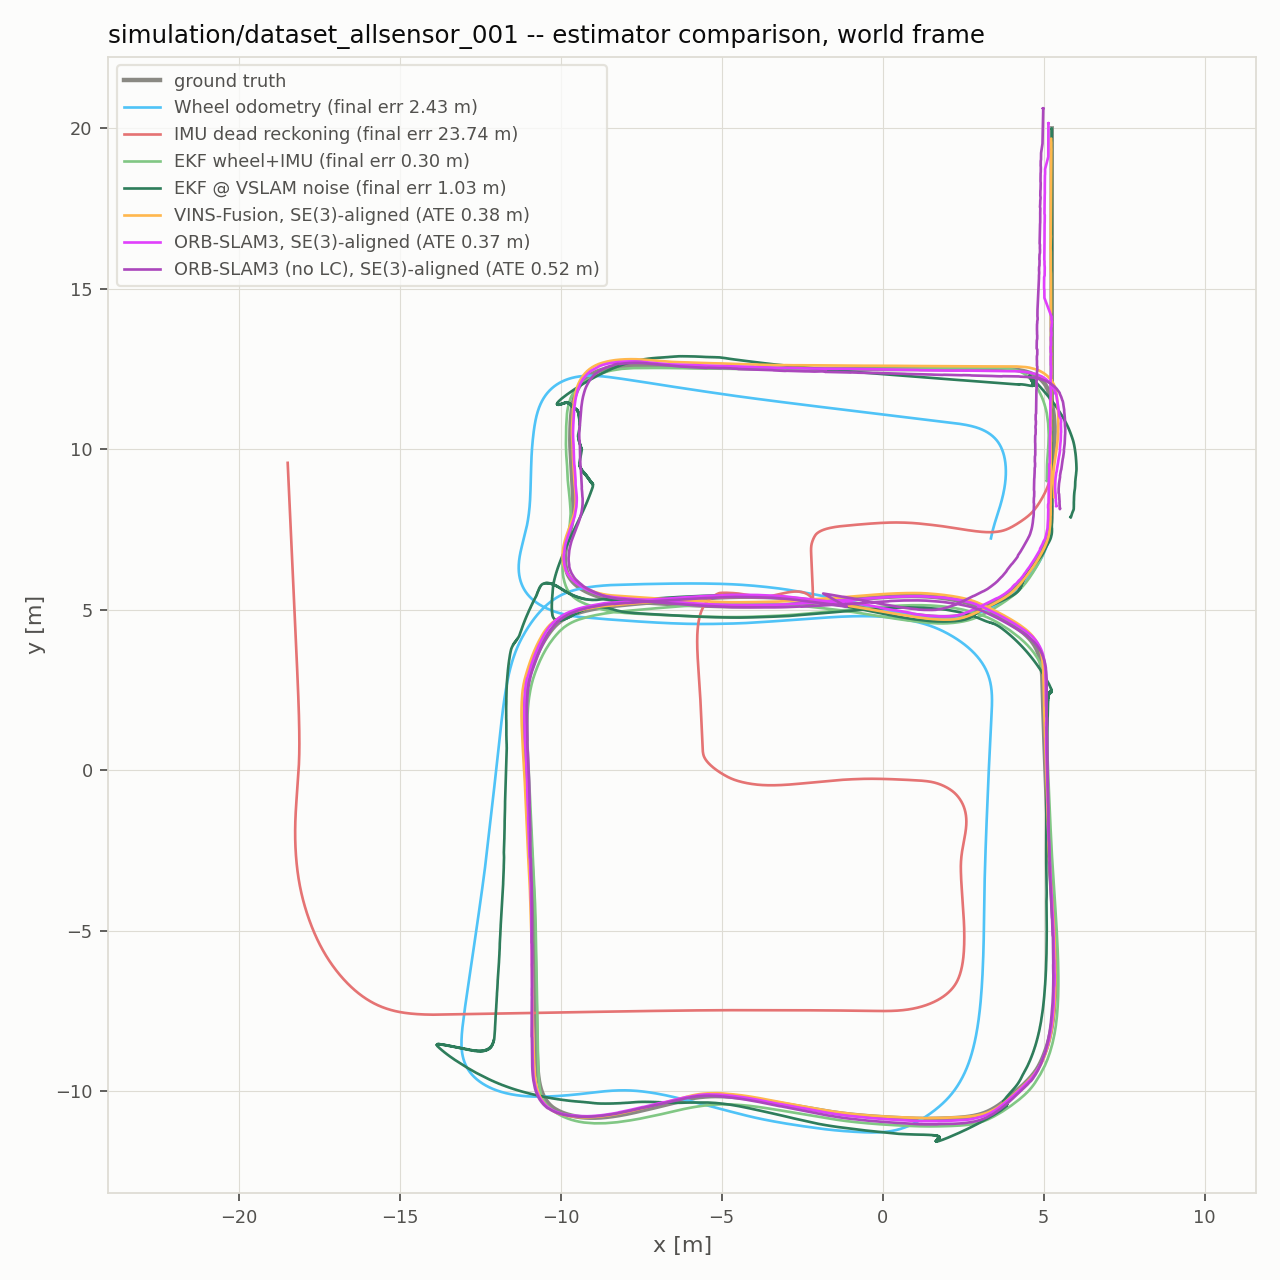
\includegraphics[width=0.82\textwidth]{../../../output/compare/simulation/exp-estimator-baseline/proprio_trajectories_dataset_allsensor_001_light.png}
  \caption[Estimator comparison on \repo{dataset_allsensor_001}, world frame.]{Estimator comparison on \repo{dataset_allsensor_001}, world frame. The
  baselines are drawn as estimated; the visual estimators are drawn after the same
  rigid $SE(3)$ alignment used for their metrics, because their own world frames
  are arbitrary. Ground truth is hidden beneath the EKF, VINS and ORB traces for
  most of the run. Wheel odometry (blue) bows consistently outward; IMU dead
  reckoning (red) leaves the building.}
  \label{fig:proprio-trajectories}
\end{figure}

\subsubsection{Falsification of H1, and the drift mechanism}
\label{sec:h1-falsified}

H1 is \flag{falsified} across all five datasets. If drift followed the fitted
yaw-rate scale, the bag with the most nearly correct scale would drift least. The
opposite holds (\cref{tab:h1}): \repo{allsensor_002} has the best scale of the
five, $+0.34\%$, and \SI{-30.11}{\degree} of heading error, while
\repo{allsensor_004} has the worst scale, $-7.50\%$, and only
\SI{-17.68}{\degree}. All five heading errors share a sign; the scale errors do
not.

\begin{table}[htbp]
\centering
\caption[Wheel-odometry heading drift against the fitted yaw-rate scale.]{Wheel-odometry heading drift against the fitted yaw-rate scale.
``Rotation'' is the total unsigned ground-truth rotation of the run, and
``error/rotation'' expresses the final heading error as a fraction of it. Scale
error and heading error correspond in neither sign nor magnitude. The last column
is the constant-offset prediction described below: the mean yaw-rate residual of
the run multiplied by its duration, which matches the measured error to within
\SI{1.4}{\degree} on every dataset, and to within \SI{0.5}{\degree} on three of
five.}
\label{tab:h1}
\small
\resizebox{\textwidth}{!}{%
\begin{tabular}{lrrrrr}
\toprule
Dataset & Yaw-rate scale & Final yaw error & Rotation & Error/rotation &
  Offset prediction \\
 & [\si{\percent}] & [\si{\degree}] & [\si{\degree}] & [\si{\percent}] &
  [\si{\degree}] \\
\midrule
\repo{allsensor_000} & $+1.10$ & $-13.76$ & 536 & $-2.566$ & $-13.81$ \\
\repo{allsensor_001} & $-4.73$ & $-12.95$ & 852 & $-1.519$ & $-13.37$ \\
\repo{allsensor_002} & $+0.34$ & \flag{$-30.11$} & 865 & $-3.481$ & $-31.03$ \\
\repo{allsensor_003} & $-6.25$ & \flag{$-37.17$} & 1123 & $-3.309$ & $-38.51$ \\
\repo{allsensor_004} & $-7.50$ & $-17.68$ & 895 & $-1.976$ & $-18.03$ \\
\bottomrule
\end{tabular}}
\end{table}

The proximate mechanism is nevertheless now identified, and it is simpler than a
scale error. The wheel model's yaw rate carries a small persistent \emph{offset}
against ground truth, averaged over all moving samples: \SI{-0.00277}{},
\SI{-0.00285}{} and \SI{-0.00624}{\radian\per\second} on the three bags. Because
heading is the time integral of that rate, an offset produces an error that grows
linearly with elapsed time rather than with rotation. Multiplying each offset by
its run duration reproduces the measured error to within \SI{1.4}{\degree} on all
five datasets (\cref{tab:h1}, last column), including the two textured-floor runs
that were recorded after the mechanism was proposed. The drift is accounted for.

\begin{queried}[Corrected]
An earlier reading of this experiment proposed that the offset came from the
bicycle model averaging the two kingpin angles, since $\tan$ of a mean is not the
mean of $\tan$. That explanation is \emph{wrong} and is withdrawn. Recomputing the
yaw rate as the mean of each wheel's own bicycle-equivalent rate changes the
residual from \SI{-0.00277}{} to \SI{-0.00288}{}, from \SI{-0.00285}{} to
\SI{-0.00296}{}, and from \SI{-0.00624}{} to \SI{-0.00630}{\radian\per\second}---
under \SI{4}{\percent} in every case, two orders of magnitude short of what the
observed drift requires. The averaging is not the source.
\end{queried}

What remains open is the origin of the offset itself. It is not a pure magnitude
error: splitting the residual by turn direction gives $+0.0109$ against $-0.0142$
on \repo{allsensor_000} and $+0.0075$ against
$-0.0292$~\si{\radian\per\second} on \repo{allsensor_002}, so the model
under-rotates in both directions \emph{and} carries a directional bias on top. On
\repo{allsensor_001}, whose route returns to its starting heading, both directions
are negative and only the bias is visible. A steering-angle zero offset, an
unmodelled slip angle, and a kingpin-geometry error are all consistent with what
has been measured so far and none has been tested.

This matters beyond wheel odometry, and the two textured-floor datasets turn what
was a caveat into a measurement. The EKF observes its gyroscope bias through
exactly this wheel yaw rate (\cref{sec:proprio-method}), so a persistent offset in
the wheel rate is absorbed into the estimated bias and reappears as heading error.
\Cref{tab:ekf-coupling} shows the two tracking each other across the five
datasets: where the wheel yaw-rate scale is within \SI{1.1}{\percent} of unity the
EKF holds heading to \SI{0.42}{\degree} or better, and where it is \SI{6}{} to
\SI{7.5}{\percent} low the EKF's heading error rises roughly tenfold.

\begin{table}[htbp]
\centering
\caption[The EKF's heading error follows the quality of the wheel yaw rate it uses to observe its gyroscope bias.]{The EKF's heading error follows the quality of the wheel yaw rate it uses
to observe its gyroscope bias. The filter is no better than its rate reference,
which is the cost of making the bias observable at all.}
\label{tab:ekf-coupling}
\small
\resizebox{\textwidth}{!}{%
\begin{tabular}{llrrrr}
\toprule
Dataset & Floor & Wheel yaw scale & Wheel yaw $\sigma$ & EKF yaw RMS & EKF ATE \\
 & & & [\si{\radian\per\second}] & [\si{\degree}] & [\si{\metre}] \\
\midrule
\repo{allsensor_000} & plain & 1.0110 & 0.0659 & 0.35 & 0.190 \\
\repo{allsensor_002} & plain & 1.0034 & 0.0705 & 0.30 & 0.256 \\
\repo{allsensor_001} & plain & 0.9527 & 0.0804 & 0.42 & 0.308 \\
\repo{allsensor_003} & bayline & 0.9375 & 0.1192 & \flag{3.54} & 0.423 \\
\repo{allsensor_004} & bayline & 0.9250 & 0.0613 & \flag{3.41} & 0.494 \\
\bottomrule
\end{tabular}}
\end{table}

An earlier version of this section, written when only the three plain-floor
datasets existed, recorded that the EKF held heading below \SI{0.7}{\degree}
everywhere and inferred that the absorbed error was small. \flag{That inference
does not survive the textured-floor datasets} and is withdrawn: the coupling is
the dominant term in the EKF's heading error whenever the wheel rate is poor, and
it sets a floor on the filter's accuracy that no amount of gyroscope quality can
lift.

One prediction of the original reasoning did survive, and is visible in
\cref{fig:proprio-covariance}: wheel-odometry error stays flat at roughly
\SI{6}{\milli\metre} for the first \SI{9.5}{\second}, the initial straight run,
and only grows once the first turn begins. Turning, not distance, starts the
error; the offset then sustains it.

\subsubsection{Covariance consistency}

H4 is supported emphatically. \Cref{tab:proprio-covariance} reports the average
normalised estimation error squared,
$\mathrm{NEES}=\mathbf{e}^{\top}\mathbf{P}^{-1}\mathbf{e}$ with
$\mathbf{e}=[\Delta x,\Delta y,\Delta\theta]$, which a correctly scaled covariance
makes average 3.0, together with the fraction of the run for which the truth lies
inside the reported $k\sigma$ bounds.

\begin{table}[htbp]
\centering
\caption[Covariance consistency of the non-visual estimators.]{Covariance consistency of the non-visual estimators. A consistent filter
gives $\mathrm{ANEES}=3.0$ and $\sigma$-coverages of 0.683, 0.954 and 0.997. Every
estimator is overconfident by roughly two orders of magnitude. Neither VINS-Fusion
nor ORB-SLAM3 writes a pose covariance, so neither can be tested here.}
\label{tab:proprio-covariance}
\small
\begin{tabular}{llrrrrl}
\toprule
Dataset & Estimator & ANEES & $1\sigma$ & $2\sigma$ & $3\sigma$ & Verdict \\
\midrule
\repo{allsensor_000} & Wheel odometry & 569.4 & 0.309 & 0.390 & 0.408 & overconfident \\
 & IMU dead reckoning & 311.0 & 0.005 & 0.022 & \flag{0.043} & overconfident \\
 & EKF wheel+IMU & 64.7 & 0.426 & 0.767 & 0.879 & overconfident \\
\midrule
\repo{allsensor_001} & Wheel odometry & 263.9 & 0.015 & 0.131 & 0.187 & overconfident \\
 & IMU dead reckoning & 339.9 & 0.001 & 0.009 & \flag{0.021} & overconfident \\
 & EKF wheel+IMU & 123.2 & 0.194 & 0.439 & 0.537 & overconfident \\
\midrule
\repo{allsensor_002} & Wheel odometry & 729.4 & 0.140 & 0.143 & 0.145 & overconfident \\
 & IMU dead reckoning & 244.7 & 0.017 & 0.045 & \flag{0.147} & overconfident \\
 & EKF wheel+IMU & 114.5 & 0.193 & 0.350 & 0.501 & overconfident \\
\midrule
\repo{allsensor_003} & Wheel odometry & 406.7 & 0.260 & 0.343 & 0.459 & overconfident \\
 & IMU dead reckoning & \flag{1504.3} & 0.010 & 0.018 & \flag{0.035} & overconfident \\
 & EKF wheel+IMU & 79.1 & 0.034 & 0.291 & 0.476 & overconfident \\
\midrule
\repo{allsensor_004} & Wheel odometry & 785.0 & 0.154 & 0.157 & 0.162 & overconfident \\
 & IMU dead reckoning & 289.5 & 0.004 & 0.017 & \flag{0.044} & overconfident \\
 & EKF wheel+IMU & 78.6 & 0.254 & 0.330 & 0.570 & overconfident \\
\midrule
\multicolumn{2}{l}{\emph{consistent reference}} & 3.0 & 0.683 & 0.954 & 0.997 & -- \\
\bottomrule
\end{tabular}
\end{table}

The IMU case is the starkest: its $3\sigma$ envelope contains the truth for
between \SI{2.1}{\percent} and \SI{14.7}{\percent} of each run, and its worst
ANEES, 1504 on \repo{allsensor_003}, is the largest figure in the experiment.
A consumer weighting this estimate by its stated covariance---a costmap, a
pose-graph edge, a relocaliser gate---would trust it tens of times more than it
deserves. Wheel odometry on \repo{allsensor_002} is the single worst case in the
experiment, ANEES 785 on \repo{allsensor_004} with $3\sigma$ coverage of 0.162, which is
consistent with
the heading offset of \cref{sec:h1-falsified}: the covariance model contains no
term for a persistent rate bias, so the larger that bias, the further the claimed
uncertainty falls behind the real error. The EKF is the least bad on every
dataset, at $3\sigma$ coverage between 0.476 and 0.879, and
\cref{fig:proprio-covariance} shows why: its NEES is genuinely near 3 during the
opening straight and only departs once turning begins, which is the same moment
the unmodelled heading error appears.

\begin{figure}[htbp]
  \centering
  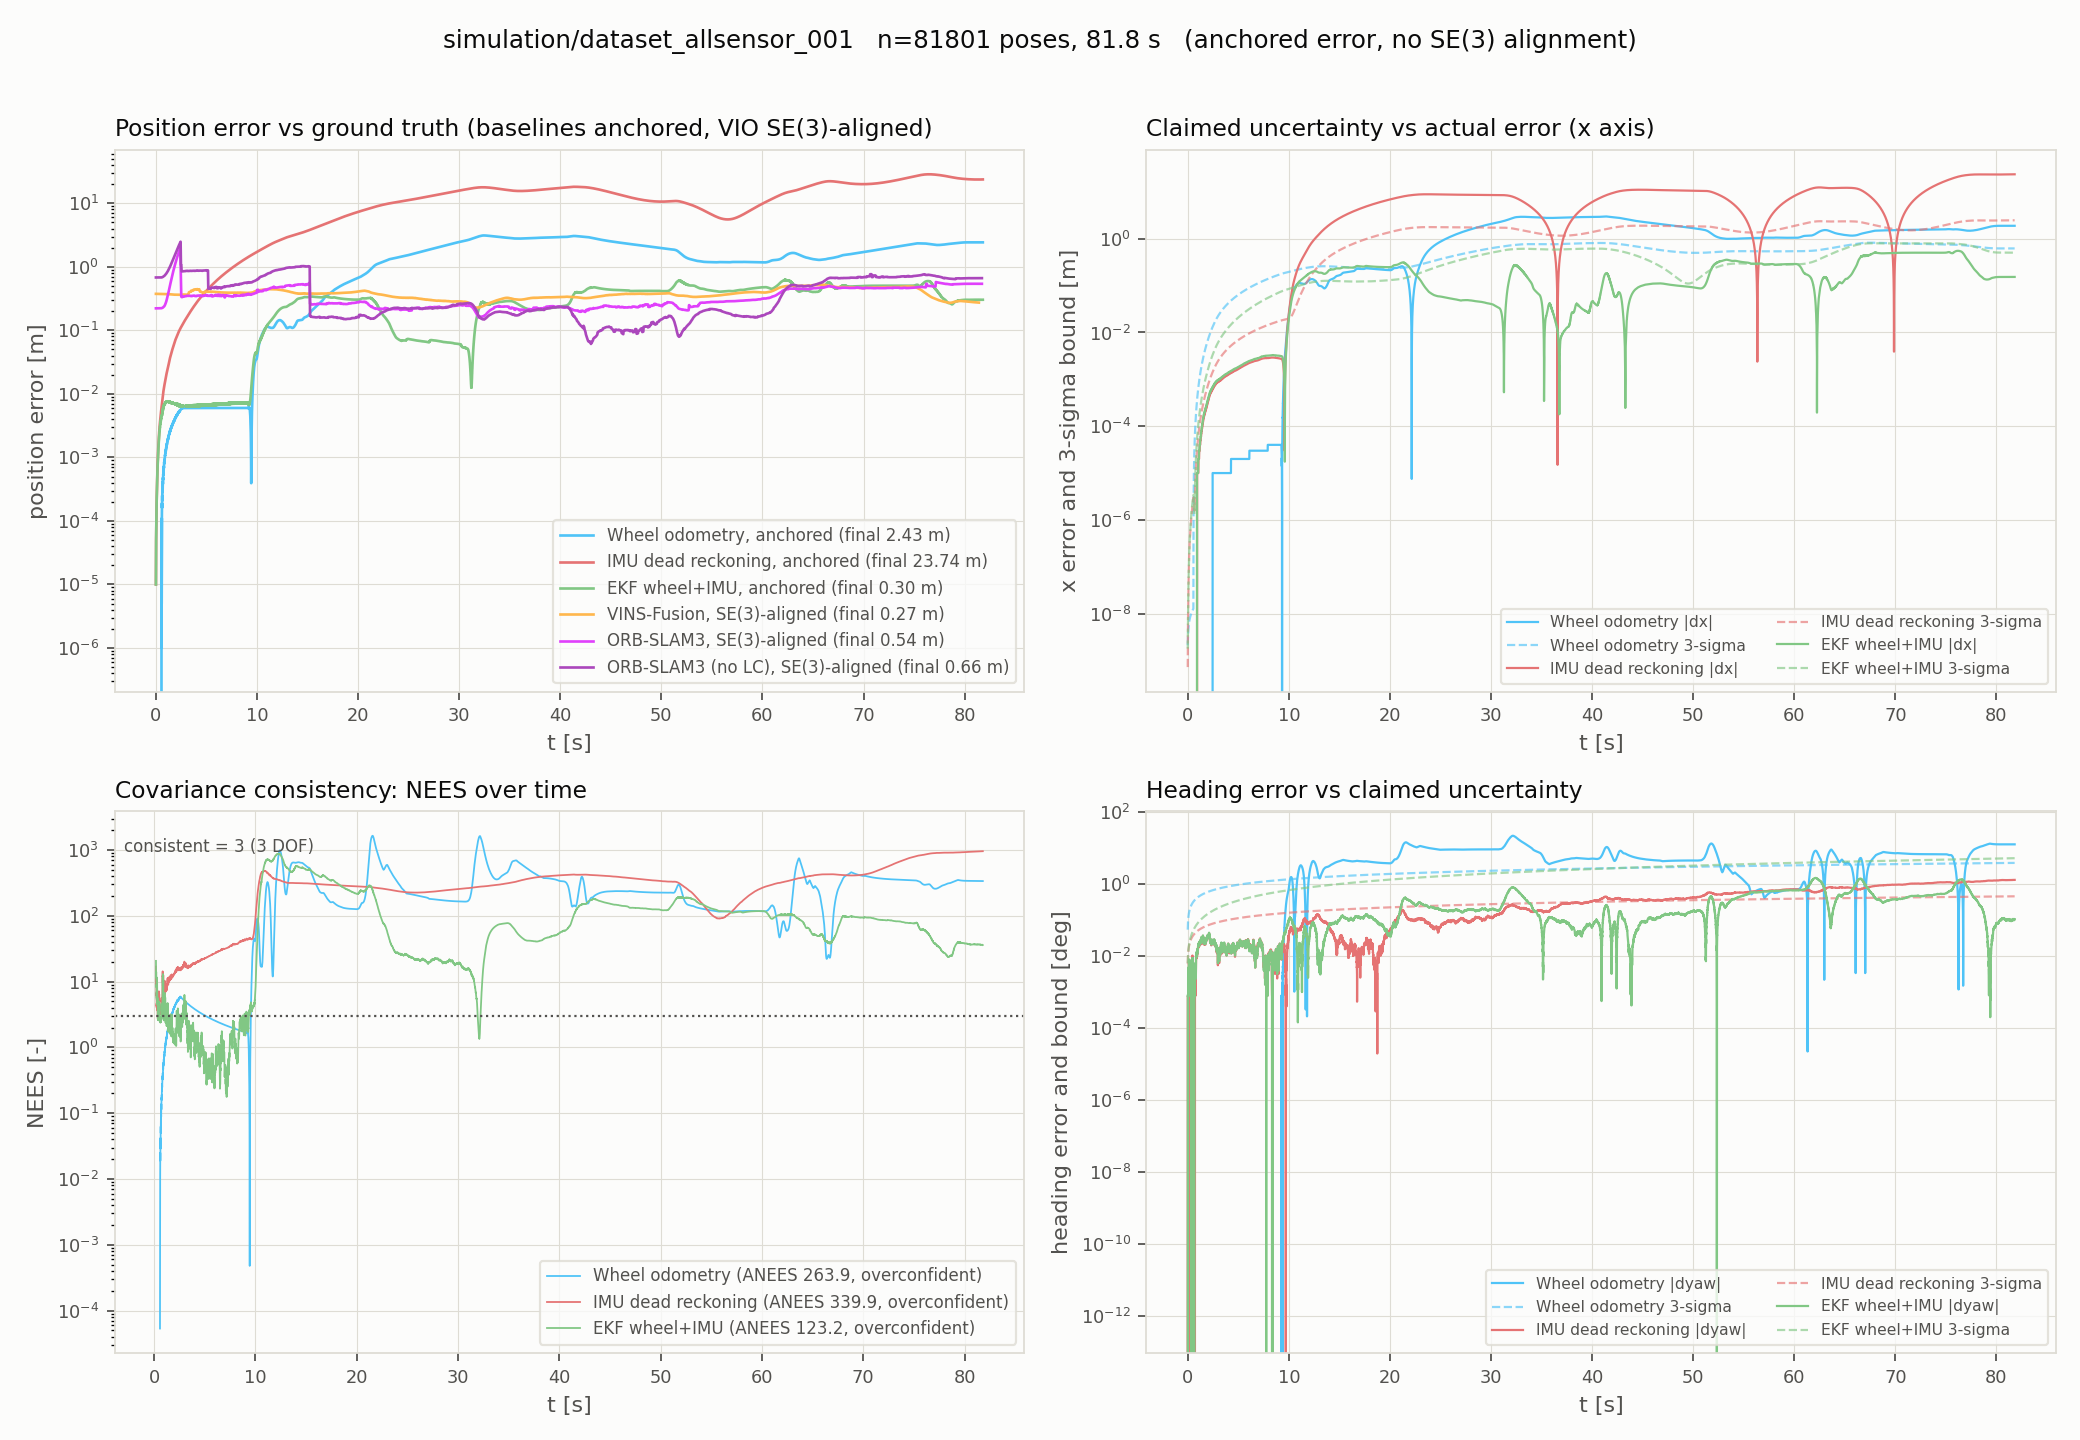
\includegraphics[width=\textwidth]{../../../output/compare/simulation/exp-estimator-baseline/proprio_covariance_dataset_allsensor_001_light.png}
  \caption[Error against claimed uncertainty for \repo{dataset_allsensor_001}.]{Error against claimed uncertainty for \repo{dataset_allsensor_001}.
  Top left: position error over time, baselines anchored and visual estimators
  $SE(3)$-aligned. Top right and bottom right: absolute error against the
  estimator's own $3\sigma$ bound, in $x$ and in heading; where the solid line
  sits above the dashed line of the same colour the filter is overconfident.
  Bottom left: NEES against the consistent value of 3. The step near
  \SI{9.5}{\second} in every panel is the first turn of the run.}
  \label{fig:proprio-covariance}
\end{figure}

\begin{queried}[Method caveat]
The $\chi^2$ interval behind the verdict column assumes independent samples. At
\SI{200}{\hertz} consecutive dead-reckoning errors are almost perfectly
correlated, so the test is run on a \SI{1}{\hertz} subsample (81 to 102 samples per dataset).
That reduces the dependence but does not remove it, and the verdicts should be
read as indicative. The $\sigma$-coverage columns make no independence assumption
and are the sturdier statement.
\end{queried}

\subsubsection{Cross-validation of the EKF noise model}

The EKF's noise model is derived from the same recording it runs on, whereas the
visual estimators receive no comparable tuning. The wheel and IMU baselines are
unaffected---their measured $\sigma$ values enter only the covariance, never the
trajectory---but the EKF's values enter the Kalman gain and so do change its
output. The comparison was therefore repeated with the noise models exchanged
between bags (\cref{tab:proprio-xval}).

\begin{table}[htbp]
\centering
\caption[EKF accuracy with an in-sample and an out-of-sample noise model.]{EKF accuracy with an in-sample and an out-of-sample noise model. The
change is negative on four of five bags---the borrowed model is \emph{better}
there---and the mean change is about $-10\%$, which is the signature of no
systematic in-sample advantage.}
\label{tab:proprio-xval}
\small
\begin{tabular}{llrr}
\toprule
Dataset & Noise model from & Aligned ATE [\si{\metre}] & Change \\
\midrule
\repo{allsensor_000} & same bag & 0.190 & -- \\
 & \repo{allsensor_001} & 0.206 & $+8.8\%$ \\
\midrule
\repo{allsensor_001} & same bag & 0.308 & -- \\
 & \repo{allsensor_000} & 0.263 & $-14.5\%$ \\
\midrule
\repo{allsensor_002} & same bag & 0.256 & -- \\
 & \repo{allsensor_000} & 0.220 & $-13.9\%$ \\
\midrule
\repo{allsensor_003} & same bag & 0.423 & -- \\
 & \repo{allsensor_000} & 0.392 & $-7.1\%$ \\
\midrule
\repo{allsensor_004} & same bag & 0.494 & -- \\
 & \repo{allsensor_000} & 0.377 & $-23.8\%$ \\
\bottomrule
\end{tabular}
\end{table}

The noise model transfers between runs, and on four of the five bags the borrowed
model is the better one, which no in-sample advantage could produce. The EKF's
accuracy is therefore a property of the estimator rather than of having seen the
answer. Cross-validated it reaches 0.206, 0.263, 0.220, 0.392 and
\SI{0.377}{\metre}, which is 1.38, 1.41, 2.53, 1.31 and 1.13 times better than the
best visual estimator of each dataset. Notably the cross-validated figure on
\repo{allsensor_004} recovers a lead that the in-sample filter did not have.

\begin{queried}[What this control does not cover]
Exchanging noise models between bags tests whether the filter saw \emph{this}
recording's answer. It cannot test the asymmetry that matters here, because both
models are still measured from data: all five bags come from one simulated IMU, so
the exchanged $\sigma$ values differ by less than a factor of two on every term
except accelerometer $x$. The visual estimators receive nothing of the kind---they
read four constants from a file. The control in \cref{sec:proprio-tuning} replaces
this one.
\end{queried}

\subsubsection{Transferring the visual systems' noise model to the EKF}
\label{sec:proprio-tuning}

\paragraph{Question and hypothesis.}
Is the EKF's advantage in \cref{tab:proprio-accuracy} an estimator effect or a
noise-model effect? Stated as a falsifiable hypothesis, \textbf{H4}: the EKF's
advantage survives being given the visual systems' own IMU noise configuration.
H4 is falsified if, on that configuration, the EKF's mean aligned ATE over the
five bags is no better than VINS-Fusion's.

\paragraph{Conditions and controls.}
The asymmetry is measured against declared, not bag against bag. VINS-Fusion and
ORB-SLAM3 both read \repo{config/wil_sim/stereo_imu.yaml}, and every one of the
fifteen visual runs in \cref{tab:proprio-accuracy} records that file in its
metadata---the five VINS runs \repo{logging_20260916_01}, and the ten ORB runs
\repo{_01} and \repo{_02}---so a single hand-set configuration stands behind the
whole visual column. The cheap half of the control is therefore to re-run the
filter on that same file. It needs no new recording: the EKF reads the bags
offline.

The independent variable is the four IMU noise terms, at three levels: the
measured per-bag values, the values \repo{stereo_imu.yaml} declares, and a set of
one-term-at-a-time ablations between them. Held fixed across every condition are
the five bags, the ground truth and its interval, the filter code and commit, the
bicycle yaw-rate model, the \SI{50}{\hertz} wheel-update stride, and the
alignment convention. The accelerometer and gyroscope biases and the whole wheel
block stay at their measured values, so the IMU noise model is the only treatment;
the single exception is the $R$-only ablation described below, which moves the
wheel yaw-rate $\sigma$ by construction. Converting the file's densities to the
per-sample $\sigma$ the filter stores ($\sigma = n\sqrt{f}$,
$f = \SI{200}{\hertz}$) gives a gyroscope term 5.5 to 6.7 times the measured
value, an accelerometer term between 0.68 and 1.44 times it, and a bias random
walk ten times it.

\paragraph{Validity and sample count.}
$n=1$ run per bag per condition, thirty runs in all. The filter is deterministic
given a bag and a noise model, so repeats would be bit-identical and no
run-to-run uncertainty can be quoted; the spread reported below is across
\emph{bags}, not runs, and is given as a range rather than a standard deviation.
All thirty completed, produced the same pose counts as their measured-noise
counterparts (17\,416, 16\,364, 17\,350, 20\,477 and 20\,104), applied the same
number of wheel corrections, and were scored over the same matched interval
against the same ground truth. The measured-noise condition is the published
baseline and was not re-run. Re-scoring it through this experiment's own code
reproduces \cref{tab:proprio-accuracy} to three decimals, which is the check that
the two paths agree.

\paragraph{Results.}
Those are the \emph{EKF @ VSLAM noise} rows of \cref{tab:proprio-accuracy}.

The result reverses the section. Mean aligned ATE over the five bags rises from
\SI{0.334}{\metre} to \SI{1.135}{\metre}, a degradation on every bag without
exception. Against that figure VINS-Fusion's \SI{0.553}{\metre} wins on
\emph{five of five}, ORB-SLAM3 without loop closing (\SI{0.804}{\metre}) on four
of five, and ORB-SLAM3 with loop closing on four of five---its mean of
\SI{1.854}{\metre} is set by the \repo{allsensor_003} outlier, and its median of
\SI{0.602}{\metre} is the fairer summary. On the metric this chapter uses
throughout, run on the tuning the visual systems actually had, both visual systems
are ahead of the filter.

\Cref{tab:proprio-tuning-ablation} locates the cause. Moving the four terms one at
a time shows that the gyroscope noise density accounts for essentially all of the
damage; the accelerometer term is inert and the bias random walk contributes
little. The density enters the filter twice---as heading process noise in $Q$, and
in the bias observation's $R$ as $\sigma_{w}^{2} + \sigma_{g}^{2}$. Raising the
wheel yaw-rate $\sigma$ so that $R$ matches the transferred case exactly while $Q$
stays measured reproduces the baseline, so the damage is entirely in $Q$. A
gyroscope density $6.5\times$ too loose inflates the heading process variance
forty-fold, and because the measurement matrix touches only $v$ and $b_{\omega}$,
heading can then be corrected only through the $P_{2,3}$ and $P_{2,4}$ cross
terms---so the wheel yaw-rate residual begins steering heading instead of staying
confined to the bias. Anchored yaw RMS rises from \SI{1.60}{\degree} to
\SI{8.67}{\degree}.

Relative pose error confirms the attribution independently, and on a local metric
that no global alignment can flatter. At $\Delta=\SI{1}{\second}$ the transferred
model degrades translation from \SIrange{0.100}{0.493}{\metre} and rotation from
\SIrange{0.285}{2.262}{\degree}; the gyroscope-only ablation reaches
\SI{0.485}{\metre} and \SI{2.179}{\degree}, almost all of it, while the
accelerometer ablation is indistinguishable from the measured model to three
decimals. The $R$-only case is marginally \emph{better} than the measured model
on all three metrics and on every bag, which says the measured wheel yaw-rate
$\sigma$ is itself slightly too tight and confirms that the $R$ path is benign
rather than merely null.

\begin{table}[htbp]
\centering
\caption[Which of the four IMU noise terms costs the EKF its accuracy.]{Which of the four IMU noise terms costs the EKF its accuracy. Each row
moves one term from its measured value to the one
\repo{config/wil_sim/stereo_imu.yaml} declares, averaged over the five bags. The
last row isolates where the gyroscope term acts: it reproduces that term's effect
on the measurement noise $R$ exactly, by raising the wheel yaw-rate $\sigma$,
while leaving the process noise $Q$ at its measured value.}
\label{tab:proprio-tuning-ablation}
\small
\begin{tabular}{lrrr}
\toprule
EKF, one term moved & Anchored RMS & Aligned ATE & Anchored yaw RMS \\
 & [\si{\metre}] & [\si{\metre}] & [\si{\degree}] \\
\midrule
measured throughout & 0.484 & 0.334 & 1.60 \\
gyroscope density, $\times 6.5$ & 1.654 & 1.105 & 8.67 \\
accelerometer density & 0.479 & 0.329 & 1.60 \\
gyroscope bias random walk, $\times 10$ & 0.654 & 0.452 & 2.97 \\
all four (\emph{EKF @ VSLAM noise}) & 1.693 & 1.135 & 8.88 \\
\midrule
gyroscope density through $R$ only & 0.475 & 0.327 & 1.50 \\
\bottomrule
\end{tabular}
\end{table}

\paragraph{Interpretation.}
Two findings survive the control and one does not. ORB-SLAM3's rotational error
stays at 13.6 to \SI{16.5}{\degree} in every condition, still
\num{2.4} times worse than the handicapped filter's \SI{6.21}{\degree}, so that
result is a property of ORB-SLAM3 and not of tuning. The complementary-failure
mechanism of the two proprioceptive sensors is likewise untouched, since it does
not depend on which $\sigma$ the filter was given. What does not survive is the
ranking of the EKF against the visual estimators.

The consistency picture moves the other way, and is worth stating because it is
the one place the transferred model does better. The EKF's ANEES falls from 64.7
to 123.2 down to 12.6 to 38.3---still overconfident by more than an order of
magnitude, but far less so. A loose noise model buys a covariance closer to
honest at the cost of the estimate itself, which is the textbook trade and is the
first time this chapter has been able to show it directly.

\paragraph{Limitations.}
\begin{queried}[What the control does and does not establish]
\flag{H4 was written down after the exploratory runs had been scored, not
before.} What is reported here is a post-hoc formalisation of an exploratory
finding; the decision rule and the direction of the test were fixed before this
subsection was written, but not before the data was seen. The unanimity---every
bag, both directions, a mechanism that isolates to one term---is what makes it
worth reporting at this stage, not a pre-registered test, and a confirmatory
repeat on bags not used to form the hypothesis is the honest follow-up.

This is also an equal-handicap comparison, not an equal-effort one: both families
now run on a declared IMU noise that nobody fitted to the data. It establishes
that the EKF's advantage in \cref{tab:proprio-accuracy} is smaller than the
tuning difference between the two families, and reverses under it. It does
\emph{not} establish that the visual systems would win a symmetric comparison.
The mirror experiment---giving VINS-Fusion and ORB-SLAM3 the measured
values---requires re-recording and has not been run to a reportable standard; the
one VINS run whose metadata confirms it diverged (\cref{sec:sim-fidelity}). The
transfer is not perfectly symmetric in role either: the filter's $\sigma_{g}$ is
a scalar in a planar five-state model, whereas \repo{gyr_n} feeds three-axis
pre-integration. Finally, $n=1$ per cell is a property of a deterministic filter
and not a design choice, but it means the between-bag range is the only
uncertainty this experiment can report.
\end{queried}

\subsubsection{Interpretation and limitations}

Across these five recordings, a five-state planar filter over wheel encoders and a
gyroscope localises more accurately than either stereo visual-inertial system
\emph{when its noise model is calibrated per bag and theirs is not}. Under the
tuning control of \cref{sec:proprio-tuning} that ordering reverses on every bag,
so the uncomfortable result for the thesis premise is weaker than it first
appeared: what these bags demonstrate is that the noise model is worth more than
the architecture over this range, not that dead reckoning outperforms vision. The
practical reading is unchanged in one respect and sharpened in another. It still
does not show that vision is unnecessary, and the justification for it still has
to come from capabilities dead reckoning does not have at all---loop closure,
relocalization after tracking loss, and the map itself---or from conditions these
bags do not contain. It now also shows that the visual systems have never been
tuned to this platform, which is the cheapest remaining source of improvement and
is the first item of \cref{sec:results-discussion}.

\begin{queried}[Generalisation limit]
The comparison is confined to \emph{static} scenes. Four worlds and both floor
conditions are now covered and the ranking is stable across them, so the earlier
form of this limitation---that the result held only on featureless floors, vision's
worst case---is no longer the binding one. \flag{Adding the bay markings did not improve
either visual estimator}, which removes that explanation rather than confirming
it---though the markings are a much weaker manipulation than ``textured floor''
suggests (\cref{fig:floor-treatments}), so a genuinely textured surface remains
untested.

What remains is that every dataset carrying wheel encoders is static
(\cref{tab:dataset-registry}). The result must not be restated as
``proprioception outperforms visual SLAM'' without that qualifier, and it cannot
be extended to dynamic scenes---where wheel odometry is unaffected by moving
objects, and where the visual systems' known failures occur---until the
\repo{allsensor} topics are recorded in a dynamic world. That recording remains
the single most informative next run in this line of work.
\end{queried}

\begin{queried}[Queried]
Both visual estimators replayed their bags at $0.5\times$ real time, so each frame
received roughly twice the wall-clock budget it would have online. The accuracy
figures in \cref{tab:proprio-accuracy} are therefore not evidence of real-time
capability, and no timing conclusion may be drawn from this experiment. The three
baselines, being offline, have no replay rate at all, which is a second asymmetry
in the same comparison.
\end{queried}

\begin{queried}[Statistical limit]
$n=5$ across four worlds, and no condition is repeated more than twice. The tables
therefore report individual values deliberately; no mean, standard deviation or
confidence interval is computed, and between-dataset differences are not evidence
of a systematic effect. A single run per world cannot establish a scene-content
effect; it shows only that the estimator ranking survives changes of scene.
\end{queried}

\begin{queried}[Unmeasured variance]
ORB-SLAM3 is multi-threaded and not deterministic, and its run-to-run spread on
identical input has not been measured here: each of its two configurations was run
once per dataset. Several differences this chapter reports sit within a range that
spread could plausibly cover---most sharply \SI{6.481}{\metre} with loop closing
enabled on \repo{allsensor_003} against \SI{0.515}{\metre} with it disabled, and
the reversal on \repo{allsensor_002} where disabling it is three times
\emph{worse}. Those differences are real measurements of the runs that were made,
but they cannot yet be attributed to the loop-closing switch. Three or more
repeats per configuration, reported as median and spread in the manner of the
relogged campaign (\cref{sec:results-validity}), are required before any
loop-closure conclusion is drawn.
\end{queried}

Two further limitations are structural rather than queried. All three baselines
begin from the ground-truth pose, because dead reckoning has no global reference;
a deployed system would have to obtain that pose some other way, which is exactly
the relocalization problem listed as future work. And the covariance result cannot
yet be extended to the visual estimators, because neither writes a pose
covariance---adding that to VINS-Fusion's marginalisation output is an
instrumentation change, not an analysis one, and is the prerequisite for applying
this consistency test to the pipelines the thesis is actually about.
